\section{Overview}
\ess can be defined as a combination of hardware components and software systems that seamlessly work together to achieve a specific purpose; they can be dynamically programmed or have a fixed functionality set, and are often engineered to achieve their goal within a larger system. They are commonly found inside devices that we use on a daily basis, such as cell phones, traffic lights, and appliances; here, these systems are responsible for controlling the functions of the device, and they are required to work continuously without the need for human intervention, besides the occasional battery replacement/recharge.
This requirement implies that, in most circumstances, providing maintenance to \ess is challenging or straight up unfeasible; therefore, the design process of a system of this kind must account for a series of additional challenges and constraints, that are typically not considered as much in \noess, in order to ensure their ability to operate in a stand-alone manner and in a wide range of conditions. Many \ess, in fact, are deployed into physical environments that do not have access to a network or are not covered by an internet connection, or are even subject to harsh and adverse weather conditions.
Furthermore, many \ess are used in applications that require a high degree of safety and security, such as in the aerospace or medical industries, meaning that the system must be able to operate without fail and without compromising safety. 

Despite the many challenges, in recent years, \ess have seen a steep surge in popularity, and have driven innovation forward in their respective areas of interest: everywhere, spanning from the agricultural field, to the medical and energy ones, \ess of various size and complexity are employed, especially in areas where human intervention is impractical or straight up impossible.
As the demand for more advanced and sophisticated devices continues to increase, the role of \ess will only become more prominent.



This requires the use of embedded software, which is specifically designed to run on the limited hardware of the system.

There are many types of \ess, including microcontrollers, digital signal processors (DSPs), and field-programmable gate arrays (FPGAs). Each of these types of systems has its own unique characteristics and is suited to different types of applications.





\section{Enabling technologies}
\subsection{Microcontrollers}
One of the key enabling technologies for \ess is their microcontroller, which is a small single-chip computer that is used to manage the functions of the larger system, in a power-efficient way and ideally at a low cost. While some applications require their own custom-made microcontroller and other custom hardware components built ad-hoc for them, there is a wide variety of general-purpose microcontroller boards, sensors, and actuators that are far easier to program and can also be customized for a high range of applications, which makes them highly versatile.

One type of general-purpose microcontroller that is commonly used for \ess development, as well as for many other IoT purposes, is the Arduino; it is an open-source platform that is based on the Atmel AVR microcontroller; it is widely used in hobbyist and educational projects because of its simplicity and low cost. Many Arduino versions exist, each with a different form factors, amounts of resources on board and I/O pins; as a result they used for applications of increased complexity and needs. Some examples include the Arduino Nano, with the smallest form factor among the Arduino boards and very limited, the Uno, and the Mega.


Another popular general-purpose microcontroller platform is the Raspberry Pi, a small single-board computer that is based on the ARM architecture, which is also what many mobile processors are based on. It comes in different variants, from an Arduino Nano-sized Raspberry Pi Zero and Zero W, but equipped with much more resources, to the Pi 3 and 4 models, which are effectively capable of running a more complex OS, supporting even up to 8GB of RAM.

In addition to these general-purpose microcontrollers, there are also many proprietary devices that are designed for specific applications: given this high specialization, these microcontrollers often offer limited customization capabilities, and may not be easily programmable, if at all, by the user. Some examples of proprietary microcontrollers include the Microchip PIC and the Texas Instruments MSP430; these chips are often used in industrial and commercial applications, where a high level of performance and reliability is required. They may also be used in applications where security is a concern, as their design may be kept confidential to protect against tampering or reverse engineering attempts.

Overall, the choice of microcontroller for an \es will depend on the specific requirements of the user. General-purpose microcontrollers such as Arduino and Raspberry Pi may be suitable for hobbyist or educational projects, while proprietary microcontrollers may be better suited for industrial or commercial applications where performance and reliability are critical.


\subsection{Embedded software and communication protocols}
Software-wise, more complex \ess can be equipped with their own \textbf{Embedded Operating System} (EOS), specifically designed to run on embedded devices, as they have a smaller footprint and fewer features compared to general-purpose OSs like Windows or Linux, and are optimized  for low power consumption. Popular EOSs include TinyOS and Embedded Linux.
Furthermore, the real-time requirements of some \ess calls for their own \textbf{Real-Time Operating System} (RTOS); these are specialized OSs that are designed to provide a predictable response time to events, even when there are many tasks running concurrently. RTOS are essential for \es that require fast and reliable performance, such as in aircraft control systems or medical devices. A notable and open-source example is FreeRTOS. 


At the lower level, communication between different components is crucial for the proper functioning of the system; there are various communication protocols that allow transmission and exchange of data, with the most notable ones being UART, I2C, and SPI:
\begin{itemize}
    \item \textbf{Universal Asynchronous Receiver/Transmitter (UART)}: one of the simplest protocols used for serial communication between devices; it is full-duplex, which means that data can be transmitted and received at the same time. UART is widely supported by many microcontrollers and microprocessor devices, however, it is typically slower than other communication protocols and can be less reliable over longer distances.
    \item \textbf{Inter-Integrated Circuit (I2C)}: a two-wire communication protocol that is used for communication between devices on the same circuit board; it is a half-duplex protocol, so data can only be transmitted or received at a time. I2C is commonly used to connect devices such as sensors, displays, and memory to a microcontroller. It is relatively fast and can support multiple devices on the same bus; however, it still has a limited data rate.
    \item \textbf{Serial Peripheral Interface (SPI)}: a two-wire communication protocol used for communication between devices; it is a synchronous protocol, which means that data is transmitted and received in a coordinated manner. SPI is relatively fast and can support multiple devices on the same bus, however, it requires more wires and pins compared to I2C and as a reseult can be more complex to implement.
\end{itemize} 


Besides communication between different components sharing the same circuit, multiple devices are often deployed as part of a larger system and must be able to efficiently communicate between each other to achieve their purpose; therefore, it is essential for \ess to be equipped with a robust suite of wireless communication protocols. As always, determining which protocol to employ depends on the constraints the system is dealing with, such as being limited to a low power consumption or being required to maintain a low-latency communication.

Zigbee is a wireless communication protocol specifically designed and built for low-power, low-data-rate applications \cite{Zigbee}; it is often used in sensors and other devices that need to communicate over short distances, such as in home automation systems or industrial control systems. Its very low power consumption makes it so ZigBee is one of the most well-suited protocols for use in devices that need to operate for long periods of time without access to a power source (\ie a quite substantial subset of \ess).
Bluetooth is another wireless protocol that is commonly used in \es which was designed for medium-range communication and is most commonly used to connect devices such as phones, tablets, and laptops to other devices, such as speakers, keyboards, or headphones. Bluetooth is a widely supported standard and is often used in applications where compatibility with a range of different devices is important; furthermore, with its low-energy variant, Bluetooth can help further optimize power consumption in devices that require it.
LoraWAN and SigFox on the other hand, are two Low-Power, Wide-Area (LPWA) communication protocol designed for IoT and machine-to-machine (M2M) applications; a typical use case is the transmission of small amounts of data over long distances, making them well-suited for use in remote monitoring systems or other applications where conventional communication methods are not practical.
For network communications, IP, and it's low energy version 6LoWPAN, are widely used protocols; they are exercised for transmitting data between devices at the network level and are a key component of the Internet.
Finally, at the application level, lightweight messaging protocols such as the Message Queue Telemetry Protocol (MQTT) are a common choice.





\section{Design challenges}
From a design and development standpoint, working with \ess can be complex, as it involves a wide range of skills and disciplines, including computer science, electrical engineering, and mechanical engineering. It is often necessary to work closely with other team members, for both the hardware and the software, to ensure that the system meets all of its requirements, functional and especially non-functional. 
In view of this, the main challenge resides in balancing the trade-offs between performance, power consumption, and cost.
For example, increasing the performance of an \es in order to accommodate a certain functionality's needs may require more power-hungry components, thus increasing the cost of the system and potentially conflicting with another requirement, according to which the device must be able to operate on a battery for long periods of time. Similarly, reducing power consumption to reach a power target may come at the expense of performance. 

Going through multiple hardware revisions in order to meet the requirements and fine-tune power and computational behavior iteratively can be extremely expensive. For this reason, as we discussed, general-purpose microprocessors should be considered in initial design phase; in most real systems however, there is the need for custom-made hardware, tailored according to the system's requirements, for security and reliability reasons.
Regardless of the microcontroller, optimization steps can be performed in most cases and involve using specialized programming languages and techniques, such as RTOSs and low-level hardware access, implementing power-saving modes and using low-power components to minimize power consumption.

Handling failures in \ess is another critical aspect to consider during their design phase: any failure should always be evident and identifiable quickly (a heart monitor should not fail quietly) \cite{MakingEmbeddedSystems}. Given the high criticality of many such systems, ensuring their dependability over the course of their lifespan is essential; \ess can be deployed in extreme conditions (\ie weather monitoring in extreme locations of the planet, satellite managements systems, devices inside the human body, and so on), where maintenance operations cannot be performed regularly, and high availability is expected. 
The dependability of an \es can be expressed in terms of:
\begin{itemize}
    \item \textbf{Maintainability}: the extent to which a system can be adapted/modified to accommodate new change requests. As \ess becomes more complex and feature-rich, it is becoming increasingly important to design them with maintainability in mind. This includes designing systems that are easy to update and repair, as well as ensuring that they can be easily replaced if necessary.
    \item \textbf{Reliability}: the extent to which a system is reliable with respect to the expected behavior. To improve reliability, \es should be designed with robust error-detection and correction mechanisms.
    \item \textbf{Availability} is the degree to which an \es is operational and accessible to its users; important for systems that are used in critical applications, such as transportation or medical equipment. To improve availability, \ess should be designed with multiple levels of redundancy and with robust fault-tolerance mechanisms. Additionally, it is important to ensure that the system is able to handle the challenges of limited bandwidth, high latency, and unreliable connectivity.
    \item \textbf{Security} refers to the ability of a system to protect against unauthorized access, modification, or destruction of data; important for systems that handle sensitive information, such as financial transactions or personal data. In order to improve security, \ess should be designed with robust encryption, security protocols, and authentication mechanisms, and should be thoroughly tested for vulnerabilities.
\end{itemize}

These dependability attributes cannot be considered individually, as there are strongly interconnected; for instance, safe system operations depend on the system being available and operating reliably in its lifespan. Furthermore, an \es can be unreliable due to its data being corrupted by an external attack or due to poor implementation. As usual, ensuring the validity of these dependability attributes in a real system, with respect to \es constraints requires trade-offs and compromises.





\section{Testing Embedded Systems}
Testing \ess poses a series of additional challenges compared to traditional systems: first, in the case of \ess that are highly integrated with a physical environment (such as with Cyber Physical Systems, CPSs), replicating the exact conditions in which the hardware will be deployed may be difficult; additionally field-testing of these systems can be unfeasible to dangerous or impractical environmental conditions (\eg a nuclear power plant, a deep-ocean station, or the human body). Secondly, given the absence of a user interface in many cases, the lack of immediate feedback makes the outcomes of the tests less observable. Moreover, resource constraints may not allow developers to fully deploy the testing infrastructure on the target hardware and thus slowing down further the process by impeding or delaying automation and regression testing. The hardware and software heterogeneity proper of \ess can also make it difficult to test them in a consistent and repeatable way. Finally, the testing of time-critical systems has to validate the correct timing behavior which means that testing the functional behavior alone is not sufficient.


\subsection{X-in-the-loop}
To mitigate some of these issues and approach \es testing in an incremental manner which allows engineers to only focus on one aspect at a time, the general testing process of \ess follows the X-in-the-loop paradigm \cite{DBLP:journals/software/GarousiFKY18}, according to which the system goes through a series of steps that simulate its behavior with an increased level of detail, before being effectively deployed on the bare hardware; subcategories in this area include Model-in-the-Loop, Software-in-the-Loop, Processor-in-the-Loop, and Hardware-in-the-Loop:
\begin{itemize}
    \item With \textbf{Model-in-the-Loop (MIL)} or \textbf{Model-Based Testing} an initial model of the hardware system is built in a simulated environment; this coarse model captures the most important features of the hardware system by using mathematical models \cite{XLoop}. As the next step, the controller module is created, and it is verified that the controller can manage the model, as per the requirements. Commonly, after the testers establish the correct behavior of the controller, its inputs and outputs are recorder, in order to be verified in the later stages of testing.
    \item With \textbf{Software-in-the-Loop (SIL)}, the algorithms that define the controller behavior are implemented in detail, and used to replace the previous controller model; the simulation is then executed with this new implementation. This step will determine whether the control logic, \ie the controller model can be actually converted to code and, perhaps more importantly, if it is hardware implementable. Here, the inputs and outputs should be logged and matched with those obtained in the previous phase; in case of any substantial differences, it may be necessary to backtrack to the MIL phase and make the necessary changes, before repeating the SIL step. On the other hand, if the performance is acceptable and falls within the acceptance threshold, we can move to the next phase.
    \item The next step is \textbf{Processor-in-the-Loop (PIL)}; here, an embedded processor, the one with which the microcontroller on the target hardware is equipped, will be simulated in detail and used to run the controller code in a closed-loop simulation. This can help determine if the chosen processor is suitable for the controller and can handle the code with its memory and computing constraints. At this point, developers have a general idea about how the embedded software will run on the hardware.
    \item Finally, \textbf{Hardware-in-the-loop (HIL)} is the step performed before deploying the \es to the actual target hardware. Here, we can run the simulated system on a real-time environment, such as SpeedGoat \cite{SpeedGoat}. The real-time system performs deterministic simulations and has physical connections to the embedded processor, \ie analog inputs and outputs, and communication interfaces, such as CAN and UDP: this can help identify issues related to the communication channels and I/O interface. HIL can be very expensive to perform and in practice it is used mostly for safety-critical applications. However, it is required by automotive and aerospace validation standards. 
\end{itemize}

After all these steps, the system can finally be deployed on the real hardware. A common environment for performing the simulation steps discussed above is Simulink \cite{Simulink}; it is a graphical modeling and simulation environment for dynamic systems based on blocks to represent different parts of a system: a block can represent a physical component, a function, or even a small system. Some notable features include: scopes and data visualizations for viewing simulation results, legacy code tool to import C and C++ code into templates and building block libraries for modeling continuous and discrete-time systems.

Figure \ref{simulink_model} ...aaa

\begin{figure}[H]
    \centering
    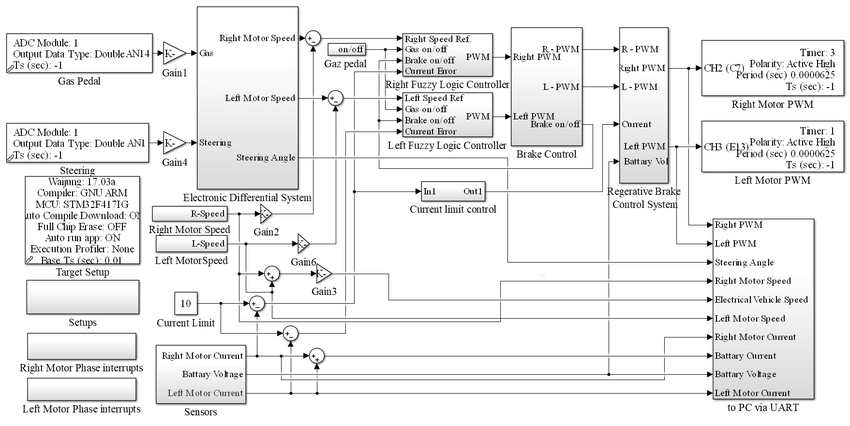
\includegraphics[width=\linewidth]{figures/simulink_model.png}
    \caption{Some components of a Simulink model for an autonomous driving system}
    \label{simulink_model}
\end{figure}


\subsection{A TDD pipeline for Embedded Systems}
Given the potential benefits of \tdd for \noess, it comes natural to ask whether this technique could be applied to the development of \ess. By applying \tdd for \ess, developers would write automated tests that would be used to verify the functionality and performance of the \es. As a reminder, these tests would be written before any code is written, and they would be used to define the requirements for the system. 
Given the higher costs of fixing issues in \ess, applying \tdd could allow developers to identify and fix problems earlier in the development process, before they become more difficult and costly to fix. It could also help to ensure that the system meets some of the requirements proper of \ess and that it is reliable, available and secure.
For the same reasons we discussed above, \tdd can be a challenging approach when applied to \ess. However, with the right tools, techniques, and experience, it is possible to apply it to \ess and to achieve the benefits of this approach. Often in fact, quality in embedded software is tied to platform-specific testing tools geared towards debugging and testing \cite{TDDEmbeddedSoftware}.
Applying TDD practices to \ess could, in theory, result in a series of benefits:
\begin{itemize}
    \item Reduce risk by verifying production code, independent of hardware, before hardware is ready or when hardware is expensive and scarce.
    \item Reduce the number of long target compile, link, and upload cycles that are executed by removing bugs on the development system.
    \item Reduce debug time on the target hardware where problems are more difficult to find and fix.
    \item Isolate hardware/software interaction issues by modeling hardware interactions in the tests.
    \item Improve software design through the decoupling of modules from each other and the hardware. Testable code is by necessity, modular.
\end{itemize}


\noindent In \cite{TDDEC}, the author proposes the "Embedded TDD Cycle", as a pipeline made of the following steps:
\begin{enumerate}
    \item \textbf{TDD micro-cycle}: this first stage is the one run most frequently, usually every few minutes. During this stage, a bulk of code is written in TDD fashion, and compiled to run on the host development system: doing so gives the developer fast feedback, not encumbered by the constraints of hardware reliability and/or availability, since there are no target compilers or lengthy upload processes. Furthermore, the development system should be a proven and stable execution environment, and usually has a richer debugging environment compared to the target platform. 
    Running the code on the development system, when it is eventually going to run in a foreign environment can be risky, so it's best to confront that risk regularly.
    \item \textbf{Compiler Compatibility Check}: periodically compile for the target environment, using the cross-compiler expected to be used for production compilations; this stage can be seen as an early warning system for any compiler incompatibilities, since it warns the developer of any porting issue, such as unavailable header files, incompatible language support, and missing language features. As a result, the written code only uses facilities available in both development environments.
    A potential issue at this stage is that in early ES development, the tool chain may not yet be decided, and this compatibility check cannot be performed: in this case, developers should take their best guess on the tool chain and compile against that compiler.
    Finally, this stage should not run with every code change; instead, a target cross-compile should take place whenever a new language feature is used, a new header file is included or a new library call is performed.
    \item \textbf{Run unit tests in an evaluation board}: compiled code could potentially run differently in the host development system and the target embedded processor. In order to mitigate this risk, developers can run the unit tests on an evaluation board; with this, any behavior differences between environments would emerge, ad since runtime libraries are usually prone to bugs \cite{TDDEC}, the risk is real. If it's late in the development cycle, and a reliable target hardware is available, this stage may appear unnecessary.
    \item \textbf{Run unit tests in the target hardware}: the objective here is again to run the test suite, however this time doing so while exercising the real hardware. One additional aspect to this stage is that developers could also run target hardware-specific tests. These tests allow developers to characterize or learn how the target hardware behaves. An additional challenge in this stage is limited memory in the target. The entire unit test suite may not fit into the target. In that case, the tests can be reorganized into separate test suites, where each suite fits in memory. This, however, does result in more complicated build automation process.
    \item \textbf{Run acceptance tests in the target hardware}: Finally, in order to make sure that the product features work, automated and manual acceptance tests are run in the target environment. Here developers have to make sure that any of the hardware-dependent code that can't be fully tested automatically is tested manually.
\end{enumerate}